\documentclass[12pt, a4paper, twoside]{book}
\usepackage[utf8]{inputenc} % Aceptar diferentes tipos de codificación de caracteres de entrada (en este caso usamos la codificación Unicode UTF-8)
%\usepackage{natbib}
\usepackage{listings}
\usepackage{eurosym}
\usepackage[spanish]{babel}
\usepackage{titlesec}
\usepackage{graphicx} % Soporte aumentado para gráficos 
\usepackage{float}
\usepackage{hyperref} % Para manejar referencias cruzadas. P.ej. añadir hiperenlaces al índice
\usepackage{caption}
\usepackage{setspace}
\usepackage{color}
\usepackage[a4paper, top=3.5cm, bottom=3.5cm, left=3cm, right=3cm]{geometry}
\spacing{1.5}
\setcounter{secnumdepth}{4}
\setlength{\parindent}{12pt}
\titleformat{\paragraph}
{\normalfont\normalsize\bfseries}{\theparagraph}{1em}{}
\titlespacing*{\paragraph}
{0pt}{3.25ex plus 1ex minus .2ex}{1.5ex plus .2ex}

%\usepackage{inconsolata}
%
%\usepackage[T1]{fontenc}
%
%\definecolor{pblue}{rgb}{0.13,0.13,1}
%\definecolor{pgreen}{rgb}{0,0.5,0}
%\definecolor{pred}{rgb}{0.9,0,0}
%\definecolor{pgrey}{rgb}{0.46,0.45,0.48}
%
%\lstset{language=Java,
%	showspaces=false,
%	showtabs=false,
%	breaklines=true,
%	showstringspaces=false,
%	breakatwhitespace=true,
%	commentstyle=\color{pgreen},
%	keywordstyle=\color{pblue},
%	stringstyle=\color{pred},
%	basicstyle=\ttfamily,
%	moredelim=[il][\textcolor{pgrey}]{$$},
%	moredelim=[is][\textolor{pgrey}]{\%\%}{\%%}
%}


\begin{document}	
	
	\thispagestyle{empty} 	
	%%%%%%%%%%%%%%%%%%%%%%%%%%%%%%%%%%%%%%%%%%%%%%%%%%%%%%%%%%%%%%%%%%%%%%%%%%%%%%%%
	% PORTADA
	%%%%%%%%%%%%%%%%%%%%%%%%%%%%%%%%%%%%%%%%%%%%%%%%%%%%%%%%%%%%%%%%%%%%%%%%%%%%%%%%
	
	\begin{center}		
		
\includegraphics[width=15cm]{Imagenes/Simbolo_logo_UDC.png}
	\end{center}
	
	% Lista de tamaños: \Huge, \huge, \LARGE, \Large, \large, \small, \footnotesize, \tiny
	\vspace{2cm}
	
	\begin{center}		
		{\textbf{ FACULTADE DE INFORMÁTICA}}
		
		\vspace{1cm}
		\LARGE{ TRABALLO FIN DE MÁSTER }	\\
		\LARGE{ MÁSTER UNIVERSITARIO EN INGENIERÍA INFORMÁTICA } \\
		\vspace{1cm}	
		\LARGE{\textbf{ Aplicación web para a xestión de menús domésticos con servizos nutricionais : Eat Fit Week! }}
	\end{center}
	
	\vspace{2cm}
	\hfill \textbf{Autor: \textit{Elías Ferreiro Borreiros}}
	
	
	\hfill \textbf{Director: \textit{Juan José Sánchez Penas}} 
	
	
	\hfill A Coruña, Agosto, 2019					
	
	\clearpage
	
	\begin{center}
		\LARGE{\textbf{ RESUMEN }}	
	\end{center}
	Hoy en día, con el cambio en los estilos de vida de las personas y tendiendo hacia unas costumbres más sedentarias, hay una mayor necesidad de enfocarse en una dieta equilibrada y saludable.
	Para ello, se han desarrollado muchos sistemas webs y móviles para la gestión de comidas y de sus valores nutricionales.	Sin embargo, analizando esos sistemas, vemos que tienen un error en su planteamiento al inundar a los usuarios con formularios sobrecargados y repletos de información innecesaria. 
	El otro problema principal de estos sistemas es la cantidad exagerada de trabajo manual que debe hacer el usuario antes de poder disfrutar de la funcionalidad principal. 
	
	Para resolver todo esto, hemos decidido plantear el desarrollo de una aplicación que solvente estos problemas y ofrezca una funcionalidad que no disponen los competidores : el análisis nutricional dinámico de las comidas planificadas para la semana configurable por el usuario. está sobrepasando.
	
	A mayores permitiremos la gestión de las entidades necesarias para esta planificación: ingredientes, platos, menús ... 
	Esto se hará siguiendo la filosofía inicial del proyecto: simplificar la entrada lo más posible y disminuir el esfuerzo requerido por el usuario. 
	Para esto llamaremos a servicios externos que nos permitirán estimar las características nutricionales de los ingredientes de forma que el usuario no tendrá que indicar esos datos y permitiremos con cada registro de usuario el alta automática de unos ingredientes base utilizables en la mayoría de recetas que agilizarán la configuración necesaria de un nuevo perfil para permitir disfrutar al máximo al usuario de las funcionalidades realmente importantes desde el momento más temprano posible.
	
	\clearpage
	
	\textbf{Título:} Aplicación web para a xestión de menús domésticos con servizos nutricionais
	\\
	\textbf{Autor:} Elías Ferreiro Borreiros
	\\
	\textbf{Tutor/Director:} Juan José Sánchez Penas
	
	
	\textbf{Palabras clave:} Java EE, POJO, Maven, Angular JS, Spring, Hibernate, Web, MySQL, Tarea, Lista, Contexto, Cliente - Servidor, Food, Planning, Management, Scrum. 
	
	
	\renewcommand{\contentsname}{Índice de contenidos}
	\renewcommand{\listfigurename}{Índice de figuras}
	\renewcommand{\listtablename}{Índice de tablas}
	
	\tableofcontents % indice de contenidos
	
	\listoffigures % indice de figuras
	
	\listoftables % indice de tablas
	
	\clearpage
	
	\chapter{Determinación de la situación actual}
	Al ser tan vital y afectar a tanto público la necesidad que solventa nuestro sistema, no somos los primeros que hemos pensado en la necesidad de tal sistema con lo que hemos podido observar que ya existen otras aplicaciones similares.
	Esto no es del todo negativo ya que nos permite evaluar otras posibles soluciones a este problema y podemos por lo tanto aprender de los errores de ellas y asimilar sus fortalezas para obtener un sistema más robusto y adecuado para esta funcionalidad.
	En el ejercicio de análisis de otras alternativas hemos seleccionado dos sistemas de gran cantidad de usuarios y por tanto de mayor interés para su evaluación:
	\section{FoodPlanner}
	FoodPlanner es un sistema de gestión de recetas con funcionalidades de planificación de comidas semanalmente / diariamente / mensualmente con funcionalidades muy similares a las que planteamos:
	\begin{center}
		\begin{figure}[H]
			\centering
			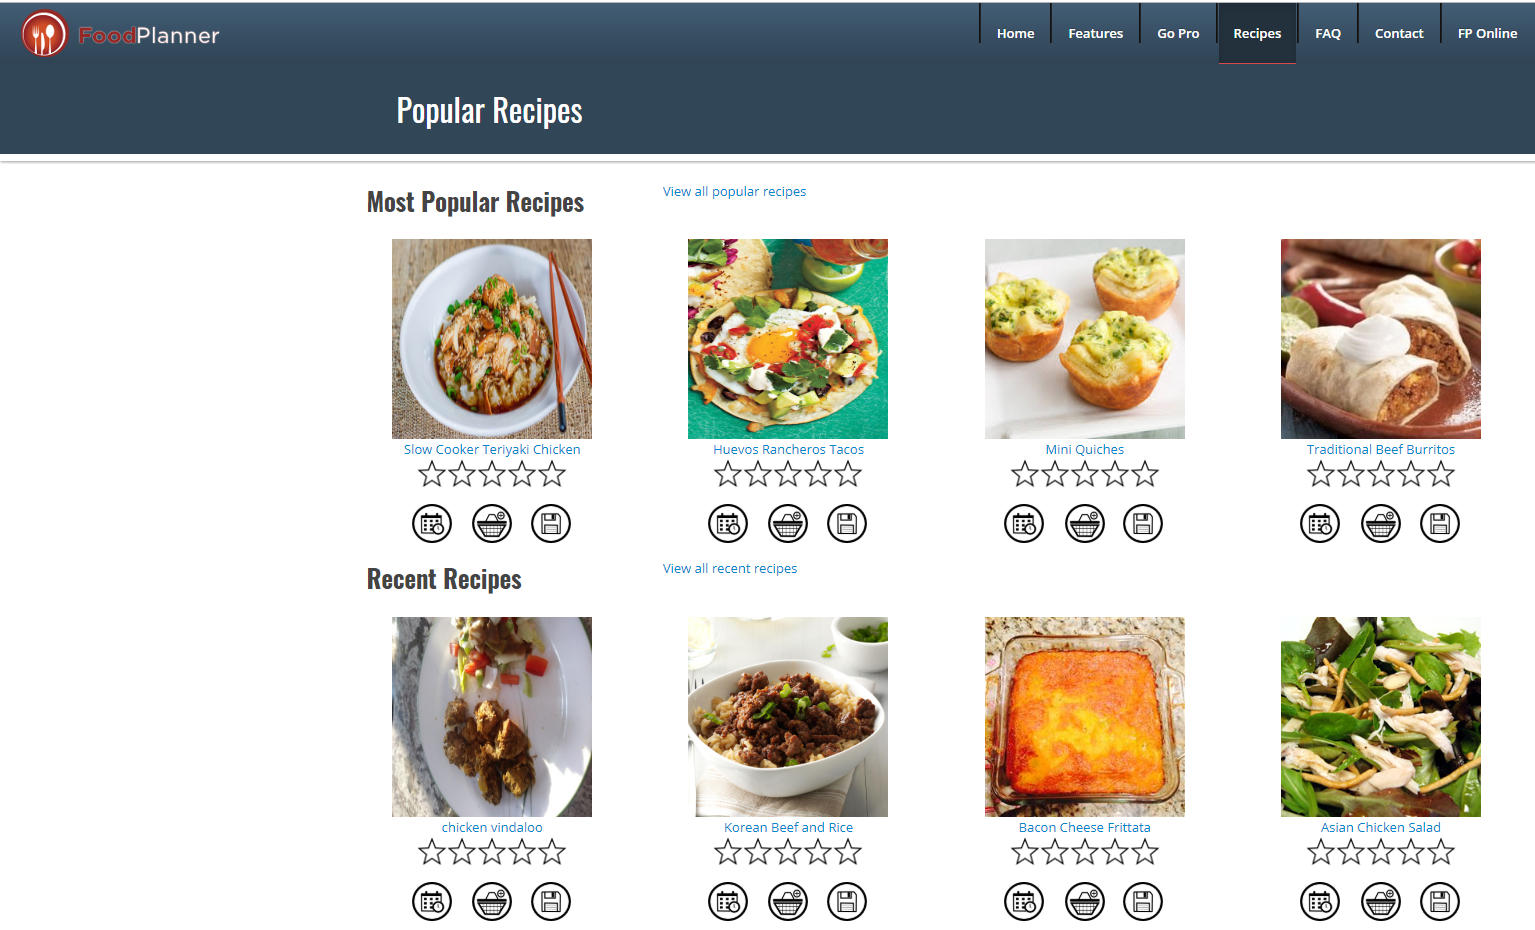
\includegraphics[width=15cm]{Imagenes/FoodPlanner.png}
			\caption{Food Planner}\label{Food Planner}
		\end{figure}
	\end{center}
	Después de una revisión del sistema y un uso del mismo como usuario podemos ver dos problemas principales que intentamos corregir con el planteamiento de nuestro sistema:
	\begin{itemize}
		\item \textbf{Excesivo trabajo necesario por el usuario para poder empezar a utilizar el sistema:} Como ejemplo, al dar de alta un plato, el sistema exige una gran cantidad de datos, a mayores, al no llevar una gestión de ingredientes, cada vez que un nuevo plato utiliza el mismo ingrediente, debemos indicarlo a mano de nuevo sin poder seleccionarlo de nuestros ingredientes registrados. Esto, sumado al hecho de que el usuario debe dar de alta todos los platos que utiliza en su día a día para poder empezar a planificar sus semanas, hace que la mayoría de los sistemas en este ámbito no se utilicen por exigir demasiado por parte del usuario y perder su interés pronto.
		\begin{center}
			\begin{figure}[H]
				\centering
				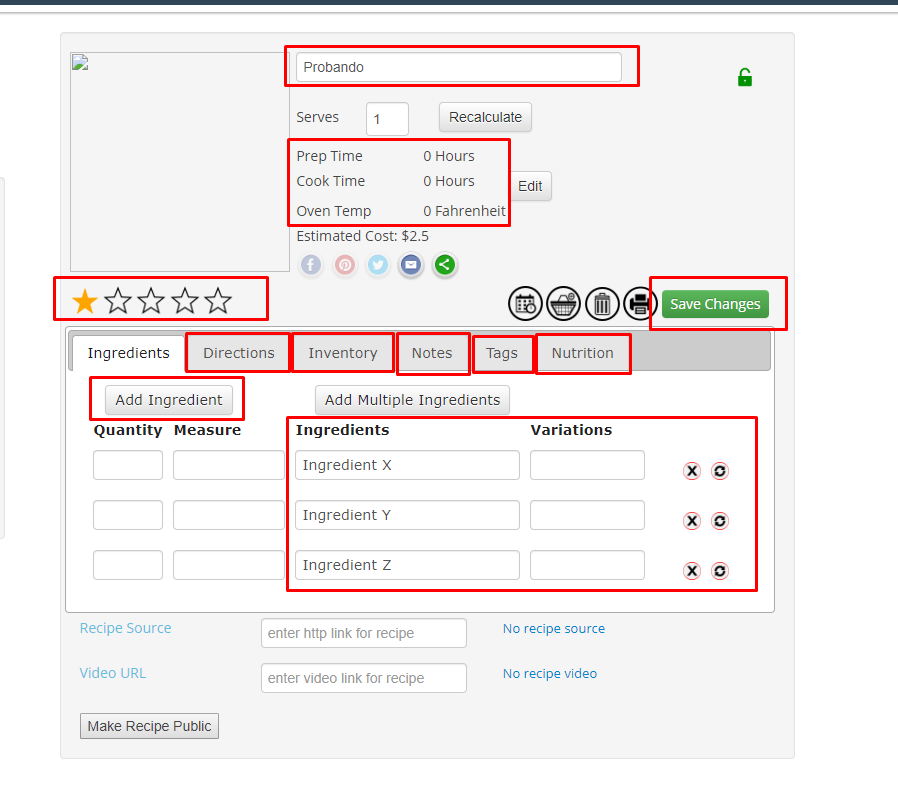
\includegraphics[width=15cm]{Imagenes/FoodPlannerAddRecipe.png}
				\caption{Food Planner Add Recipe}\label{Food Planner Add Recipe}
			\end{figure}
		\end{center}
		\textbf{Solución:} Énfasis en la sencillez en los formularios sin el requerimiento de datos innecesarios y carga de datos base comunes (Ingredientes que utilizará el usuario base en la mayoría de sus platos) en cada registro de nuevos usuarios para evitar trabajo al usuario.
		\item \textbf{Poco énfasis en las características nutricionales de los platos:} En FoodPlanner para obtener las calorías, grasas ... de un plato se requiere indicar una url con la receta de ese plato en páginas concretas seleccionadas, esto es muy laborioso para el usuario ya que para cada plato debe buscar esa receta en dichas páginas y tiene el posible problema de que no exista en esas páginas con lo que el usuario no podría tener datos nutricionales sobre su plato. A mayores, no permite visualizar en el calendario los stats nutricionales del menú actual lo que supone la funcionalidad principal del sistema que planteamos:
		\begin{center}
			\begin{figure}[H]
				\centering
				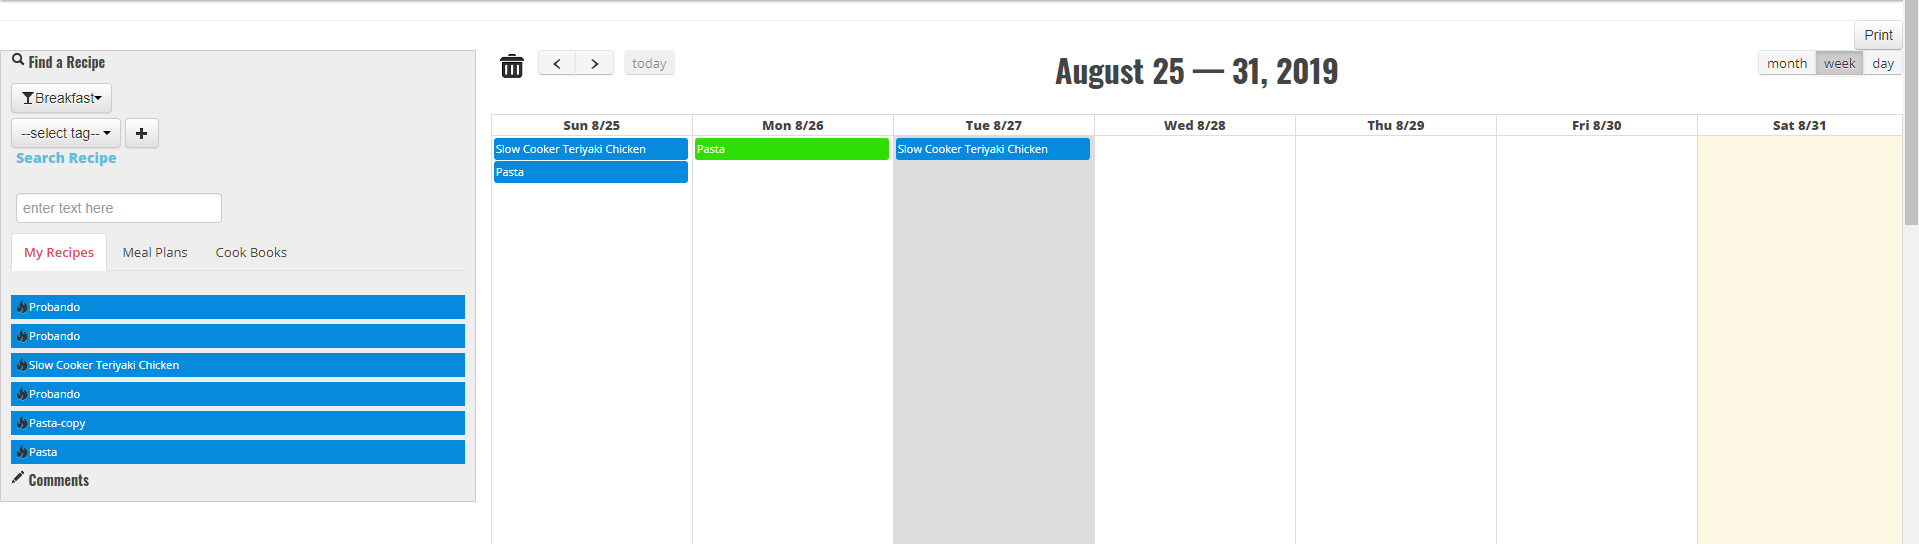
\includegraphics[width=15cm]{Imagenes/FoodPlannerCalendar.png}
				\caption{Food Planner Calendar}\label{Food Planner Calendar}
			\end{figure}
		\end{center}
		\textbf{Solución:} Llamada a un servicio automático para dar valor de stats nutricionales a los ingredientes / platos que registre el usuario pero de forma que sea transparente para él y no le requiera mayor esfuerzo. Énfasis en la visualización de estos stats en todo momento en el menú semanal para dar mayor importancia a los mismos.
	\end{itemize}	
	\section{Eat This Much}
	Así como FoodPlanner es un gestor de recetas que te permite almacenarlas y gestionar sus datos pero que no hace gran énfasis en sus valores nutricionales y su análisis, Eat This Much representa la otra cara de la moneda siendo un sistema que permite indicar las características de la dieta exigida (Calorías, Tipo de dieta, Cantidad de comidas):
	\begin{center}
		\begin{figure}[H]
			\centering
			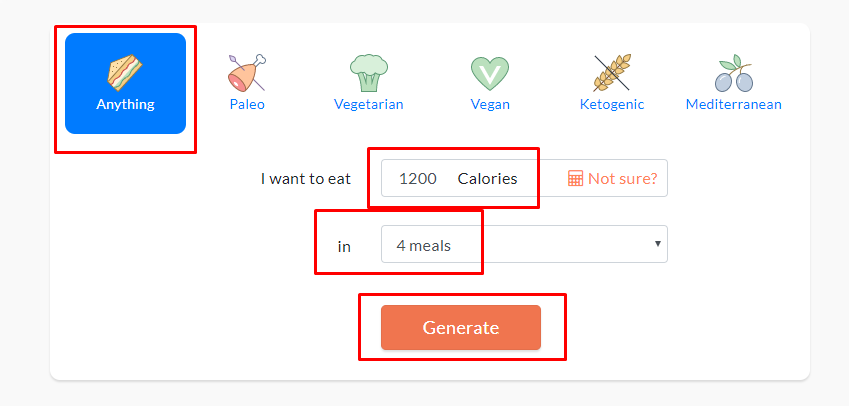
\includegraphics[width=10cm]{Imagenes/EatThisMuchSelection.png}
			\caption{Eat This Much Selection}\label{Eat This Much Selection}
		\end{figure}
	\end{center}
	Y, a partir de esas características, genera automáticamente un menú que las cumple con platos seleccionados por el sistema aleatoriamente:
	\begin{center}
		\begin{figure}[H]
			\centering
			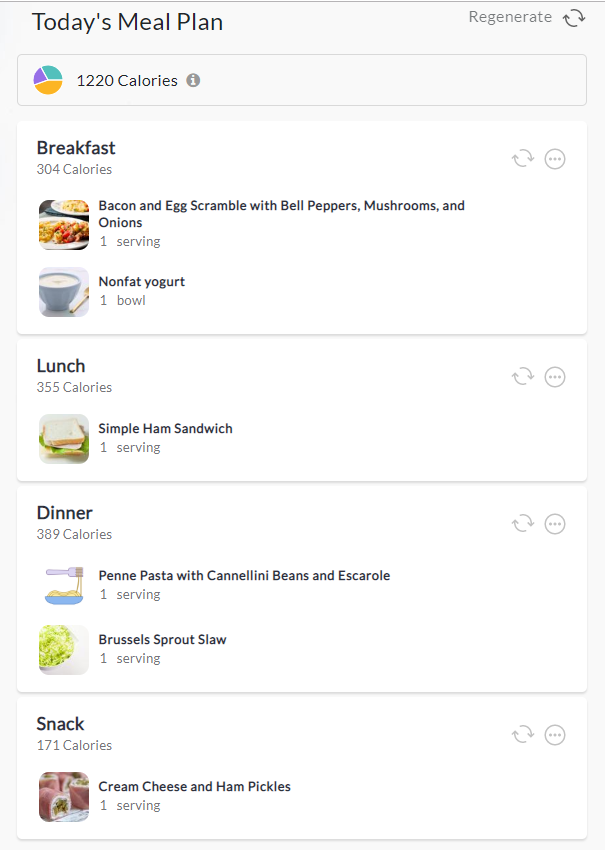
\includegraphics[width=10cm]{Imagenes/EatThisMuchMenu.png}
			\caption{Eat This Much Menu}\label{Eat This Much Menu}
		\end{figure}
	\end{center}
	El \textbf{principal problema} que vemos con este concepto de sistema es que el usuario realmente deja su menú ``a merced'' de la aplicación de forma que puede obtener menús con platos que no sabe cocinar, o bien no le gustan. Aún así, como comentábamos anteriormente, si que vemos una gran ventaja en obtener menús ``aleatorios'' que cumplan las necesidades dietéticas del usuario ya que, al ser aleatorios, evitan rutina y repetición en la dieta del usuario.\\
	Por tanto, la \textbf{principal solución} sería implementar en nuestro sistema un algoritmo de creación de menús válidos pero ÚNICAMENTE con los platos registrados por el usuario, de forma que siga teniendo el control total sobre los platos que aparecerán en sus menús semanales y no aparezcan aquellos no deseados por él.
	
	Como resumen del análisis de los dos sistemas, vemos que deberíamos intentar tomar las fortalezas de ambos para formar un sistema que, a mayores de permitir llevar un \textbf{registro de los ingredientes y platos favoritos del usuario}, haga énfasis en la \textbf{sencillez del diseño de los formularios y de la información} y permita \textbf{generar menús aleatorios acordes a las necesidades dietéticas del usuario}.
	
\end{document}

